\documentclass[]{article}

\begin{document}

\title{Title}
\author{Author}
\date{Today}
\maketitle

Architecture-Driven Modernization (ADM) ``\textit{is a process to understand and to improve existing software assets. ADM restores the value of existing applications}''. In other words, it can be stated  as a mechanism for software evolution, i.e., it makes it possible to modernize the legacy information systems and eradicates, or at least minimizes, the software erosion problem in legacy systems~\cite{OMGADM}. Also we can define ADM as a process to understand and evolve existing software assets of a system of interest. ADM focuses at collecting, sharing, utilizing, transforming, presenting, maintaining, and storing models of the architectural aspects of existing systems. The ADM aims to resolve the problems of traditional reengineering since it performs reengineering processes taking model-driven principles into account. However, it worth to notice that ADM goal is not to replace the traditional reengineering process but enhance it. 

Figure~\ref{fig:horseshoe} shows that ADM has adapted the horseshoe modernization model. As can be seen in this figure, there are the same three types of models used in Model-Driven Architecture (MDA)~\cite{ThomasMDA}: (\textit{i}) Computation Independent Model (CIM) aims to provide a  a view of the system from the computation independent viewpoint at a high abstract level, i.e., it represents the context and purpose of the system without any computational complexities; (\textit{ii}) Platform Independent Model (PIM) aims to represent the system in a independent viewpoint, i.e., normally it describes the behavior and structure of the application regardless of the implementation platform; and (\textit{iii}) Platform Specific Model (PSM) can be defined as a view of the system, i.e., usually it may not be executed but it contain all required information regarding a specific platform that developers may use to implement the executable code~\cite{Deltombe, 5440163, ThomasMDA}.

\begin{figure}[t]
\centering
  % Requires \usepackage{graphicx}
  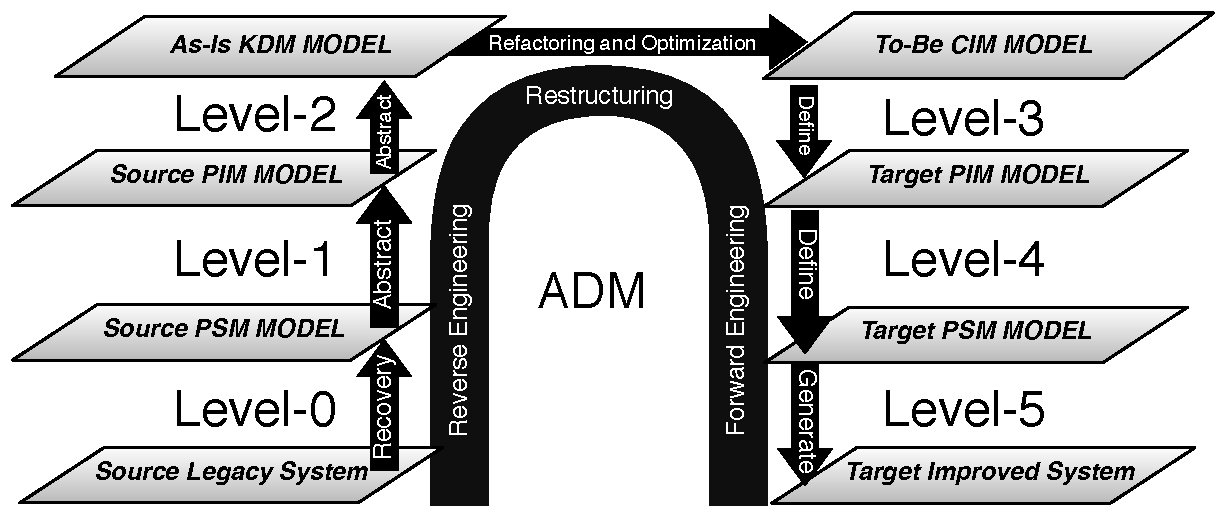
\includegraphics[scale=0.6]{Figure/processoDaFerramenta}
\caption{Horseshoe modernization model (OMG Group~\cite{OMGADM})}
\label{fig:horseshoe}
\end{figure}


Accordingly to OMG~\cite{OMGADM} one of the main aim of ADM is not only follows the principles of MDA, ADM has also set off the development of a set of standards to deal with different challenges that appear in the modernization of legacy information systems~\cite{1686216}. In this context, the ~\emph{Architecture-Driven Modernization Task Force} (\emph{ADMTF}) issued the request-for-proposal of Knowledge Discovery Meta-model (KDM).  KDM is a meta-model for representing existing software, its elements, associations, and operational environments. According to OMG and Ricardo~\cite{OMGADM, ricardo} the KDM goals is to be a meta-model to allow software engineer to create tools to exchange application metadata across different application, languages, platforms and environments. By using KDM it is also possible to aggregate or modify, i.e. refactor, the legacy system;

As stated before, the KDM is an OMG discovery meta-model specification; and nowadays it is being adopted as \emph{ISO/IEC 19506} by the \emph{International Standards Organization} for representing information related to existing software systems. Moreover, KDM is defined via \emph{Meta-Object Facility} (\emph{MOF}). KDM determines the interchange format via the \emph{XML Metadata Interchange} (\emph{XMI}) by applying the standard MOF to XMI mapping to the KDM MOF model. 
\end{document}